\documentclass[11pt]{article}

\usepackage[utf8]{inputenc}%Size of the text
\usepackage[english]{babel}%For english keyboard
\usepackage[toc,page]{appendix}
\usepackage{authblk} %pour faire une jolie première de couverture
\usepackage{amsfonts,amssymb,amsmath}%To use the mathematics environements
\usepackage{setspace} % pour définir l'interligne qu'on veut
\doublespacing % l'interligne qu'on veut (ici 1,5)
\usepackage{subcaption}


\usepackage{subcaption}%For pictures side by side
\usepackage{changepage}%For adjustwidth
\usepackage[a4paper,left=1.8cm,right=1.8cm,top=2cm,bottom=2cm]{geometry}
\usepackage{booktabs}
\usepackage{array}
\usepackage[usenames,dvipsnames]{color}%To make nice color
\usepackage[flushleft]{threeparttable}%fot table notes
\usepackage{lscape}%Pages in landscape
\usepackage[hyperfootnotes=false]{hyperref}%To change ref's settings
	\hypersetup{
		pdftitle={},    % title
		 colorlinks = true,
		 citecolor=Blue,%Color for cite
 		 linkcolor=Red,%COlor link
  		urlcolor=Blue}%Color URL
  		
\usepackage{float}%Position for figure 
\newcommand\fnote[1]{\captionsetup{font=footnotesize}\caption*{#1}}
\usepackage{adjustbox}%To wrape big table
\usepackage{multirow}%To have multicol in tabular

\usepackage{bbm}
\usepackage{graphicx}%Allows to insert graphics, prictures
\graphicspath{{figures/}} % Directory in which figures are stored
\newcolumntype{L}[1]{>{\raggedright\arraybackslash}p{#1}}
\newcolumntype{C}[1]{>{\centering\arraybackslash}p{#1}}
\usepackage{textcomp} %notamment pour utiliser un ° (degré)

\DeclareUnicodeCharacter{2212}{-}


\usepackage[sectionbib,square]{natbib}


\title{New Economic Geography Model, \\ Helpman (1998)}


\author[]{Pol Cosentino\thanks{\small{Université Paris 1 Panthéon-Sorbonne\\ \href{mailto:Pol.Cosentino@etu.univ-paris1.fr}{Pol.Cosentino@etu.univ-paris1.fr}}  
\\ This note is largely taken from Quantitative spatial economics, Redding and Rossi-Hansberg, 2017, Annual Review of Economics.}}



\date{}

\renewcommand\Authands{ and }

\bibliographystyle{apalike}

\begin{document}
\thispagestyle{empty}
\maketitle



\thispagestyle{empty}%To not count page
\newpage


\pagenumbering{arabic} \setcounter{page}{1} %start counting page at this slide


\section*{Motivation}
Canonical Quantitative Spatial Model (used in Hanson (2005) and Redding \& Sturm (2008))
\begin{itemize}
\item multiregion connected by goods trade and factor mobility
\item study the determinants of the spatial distribution of economic activity 
\end{itemize}
Components
\begin{enumerate}
\item Preferences
\begin{itemize}
\item taste for variety and common preferences
\item single traded sector
\item no amenities
\item residential land use
\end{itemize}
\item Production Technology
\begin{itemize}
\item increasing returns to scale
\item exogenous productivity
\item no input–output linkages
\item no commercial land use
\end{itemize}
\item Costs of Trading Goods
\begin{itemize}
\item iceberg variable trade costs
\item symmetric trade costs
\item economic and geographic frictions
\item no nontraded goods besides residential land use
\end{itemize}
\item Technology for Idea Flows
\begin{itemize}
\item no knowledge externalities or diffusion
\item no innovation
\item no transferability of ideas
\end{itemize}
\item Costs of Moving People
\begin{itemize}
\item perfectly costless migration
\item no commuting
\item single worker type with no heterogeneity
\item no congestion in transportation
\end{itemize}
\item Endowments
\begin{itemize}
\item homogeneous labor
\item exogenous land endowments in regions within a single country
\item no capital
\end{itemize}
\item Equilibrium
\begin{itemize}
\item general equilibrium with a single country
\item monopolistic competition
\item land rents redistributed to residents
\item balanced trade in each location
\end{itemize}
\end{enumerate}



\section*{Model set-up}
\begin{itemize}
\item wide economy of $N$ regions indexed by $n$
\item each region is endowed with an exogenous quality-adjusted supply of land ($H_{i}$) 
\item whole economy is endowed with a measure $\overline{L}$ of workers
\item each worker has one unit of labor that is supplied inelastically with zero disutility
\item workers are perfectly geographically mobile $\Rightarrow$ in equilibrium, real wages are equalized across all populated regions
\item regions are connected by a bilateral transport network that can be used to ship goods subject to symmetric \textbf{iceberg trade costs}:  $d_{ni} = d_{in} >1$ units must be shipped from region $i$ in order for one unit to arrive in region $n \neq i$, where $d_{nn}=1$
\end{itemize}

\subsection*{Consumer-Preferences}
Cobb-Douglas utility function;
\begin{equation}
U_{n} = \Big( \frac{C_{n}}{\alpha} \Big)^{\alpha} \Big( \frac{h_{n}}{1 - \alpha} \Big)^{1 - \alpha}, \quad 0 < \alpha < 1
\end{equation}
with 
\begin{itemize}
\item $C_{n}:$ goods consumption, defined over consumption $c_{ni}(j)$ of each horizontally differentiated variety $j$ from the endogenous measures $M_{i}$ supplied by each region
\item $h_{n}:$ residential land use
\end{itemize}
\begin{equation} \label{PI_CI}
C_{n} = \Big[ \sum_{i \in N} \int^{M_{i}}_{0} c_{ni}(j)^{\rho} dj \Big]^{1/\rho}, \quad P_{n} = \Big[ \sum_{i \in N} \int^{M_{i}}_{0} p_{ni}(j)^{1 - \sigma } dj \Big]^{1/1-\sigma}
\end{equation}

\subsection*{Production}
Total amount of labor $l_{i}(j)$ required to produce $x_{i}(j)$ units of variety $j$ in location $i$ taking into account fixed cost $F$ (monopolistic competition and increasing returns to scale) and location productivity $A_{i}$,
\begin{equation}
l_{i}(j) = F + \frac{x_{i}(j)}{A_{i}}
\end{equation}
Profit maximization and zero profits imply that equilibrium prices are a constant markup over the marginal cost of supplying a variety to a market,
\begin{equation} \label{equi_prices}
p_{ni}(j) = \Big( \frac{\sigma}{1 - \sigma} \Big) d_{ni} \frac{w_{i}}{A_{i}},
\end{equation}
and equilibrium output of each variety is equal to a constant that depends on location productivity,
\begin{equation}
x_{i}(j) = \overline{x}_{i} = A_{i}(\sigma - 1 ) F,
\end{equation}
which implies that equilibrium employment for each variety is the same for all locations,
\begin{equation}
l_{i}(j) = \overline{l} = \sigma F
\end{equation}
Given this constant equilibrium employment for each variety, labor market clearing implies that the total measure of varieties supplied by each location is proportional to the endogenous supply of workers choosing to locate there:
\begin{equation} \label{LM_clearing}
M_{i} = \frac{L_{i}}{\sigma F}
\end{equation}

\subsection*{Price Indices and Expenditure Shares}
Using equilibrium prices (Equation \ref{equi_prices}) and labor market clearing (Equation \ref{LM_clearing}), one can express the price index dual to the consumption index (Equation \ref{PI_CI}) as
\begin{equation}\label{equa_8}
P_{n} = \frac{\sigma}{\sigma - 1} \Big( \frac{1}{\sigma F} \Big)^{1/1-\sigma} \Big[ \sum_{i \in N} L_{i} \Big( d_{ni} \frac{w_{i}}{A_{i}} \Big)^{1-\sigma} \Big]^{1/1-\sigma}
\end{equation}
Using the constant elasticity of substitution (CES) expenditure function, equilibrium prices (Equation \ref{equi_prices}), and labor market clearing (Equation \ref{LM_clearing}), the share of location $n$’s expenditure on goods produced in location $i$ is
\begin{equation}\label{equa_9}
\pi_{ni} = \frac{M_{i} p_{ni}^{1-\sigma}}{\sum_{k \in N} M_{k} p_{nk}^{1-\sigma}} = \frac{L_{i} \Big( d_{ni} \frac{w_{i}}{A_{i}} \Big)^{1-\sigma}}{\sum_{k \in N} L_{k} \Big( d_{nk} \frac{w_{k}}{A_{k}} \Big)^{1-\sigma}}
\end{equation}
The model therefore implies a gravity equation for goods trade, where the bilateral trade between locations $n$ and $i$ depends on both bilateral resistance (bilateral trade costs $d_{ni}$) and multilateral resistance (trade costs to all other locations $k$, $d_{nk}$).\\
Together, Equations \ref{equa_8} and \ref{equa_9} imply that each location's price index can be written in terms of its trade share with itself, so
\begin{equation} \label{equa_10}
P_{n} = \frac{\sigma }{ \sigma - 1} \Big( \frac{L_{n}}{\sigma F \pi_{nn}} \Big)^{1/1-\sigma} \frac{w_{n}}{A_{n}}
\end{equation}

\subsection*{Income and Population Mobility}
Expenditure on land in each location is redistributed in a lump sum to the workers residing in that location. Therefore, trade balance at each location implies that per capita income $\nu_{n}$ in each location equals labor income $w_{n}$ plus per capita expenditure on residential land, $(1 - \alpha )\nu_{n}$,
\begin{equation} \label{equa_11}
\nu_{n} L_{n} = w_{n} L_{n} + (1-\alpha ) \nu_{n} L_{n} = \frac{w_{n} L_{n}}{\alpha }
\end{equation}
Land market clearing implies that the supply of quality-adjusted land, $H_{n}$ , equals the demand for land, $L_{n} h_{n}$.\\
By combining this market clearing condition with the FOC of the consumer problem, we obtain the result that land rents, $r_{n}$ , are given by
\begin{equation} \label{equa_12}
r_{n} = \frac{(1 - \alpha ) \nu_{n} L_{n}}{H_{n}} = \frac{1 - \alpha}{\alpha} \frac{w_{n} L_{n}}{H_{n}}
\end{equation}
Population mobility implies that workers receive the \textbf{same} real income in all populated locations,
\begin{equation} \label{equa_13}
V_{n} = \frac{\nu_{n}}{ P^{\alpha}_{n} r^{1-\alpha}_{n}}  = \overline{V}
\end{equation}
By using the price index (Equation \ref{equa_10}), the assumption that trade is balanced at each location such that income equals expenditure (Equation \ref{equa_11}), and land market clearing (Equation \ref{equa_12}) in the population mobility condition (Equation \ref{equa_13}), one determines that real wage equalization implies that the population $L_{n}$ and domestic trade share $\pi_{nn}$ of each location must satisfy
\begin{equation} \label{equa_14}
\overline{V} = \frac{A^{\alpha}_{n} H^{1-\alpha}_{n} \pi_{nn}^{-\alpha / (\sigma -1)} L_{n}^{-\frac{\sigma (1 - \alpha ) - 1}{\sigma - 1}}}{\alpha \Big( \frac{\sigma}{\sigma - 1} \Big)^{\alpha} \Big( \frac{1}{\sigma F} \Big)^{\frac{\alpha}{1 - \sigma}} \Big( \frac{1 - \alpha}{\alpha} \Big)^{1 - \alpha}}
\end{equation}
Therefore, the population share of each location ($\lambda_{n} \equiv L_{n}/ \overline{L} $) depends on its productivity $A_{n}$, supply of land $H_{n}$, and domestic trade share $\pi_{nn}$ relative to those of all other locations,
\begin{equation} \label{equa_15}
\lambda_{n} = \frac{L_{n}}{\overline{L}} = \frac{\Big[ A^{\alpha}_{n} H_{n}^{1-\alpha} \pi_{nn}^{-\alpha / (\sigma - 1)} \Big]^{\frac{\sigma - 1}{\sigma (1-\alpha )-1}}}{\sum_{k} \in N \Big[ A^{\alpha}_{k} H_{k}^{1-\alpha} \pi_{kk}^{-\alpha / (\sigma - 1)} \Big]^{\frac{\sigma - 1}{\sigma (1-\alpha )-1}}}
\end{equation}
where each location's domestic trade share $\pi_{nn}$ summarizes its market access to other locations.

\subsection*{General Equilibrium}
The properties of the general equilibrium of the model can be characterized analytically by combining the trade share (Equation \ref{equa_9}), price index (Equation \ref{PI_CI}), and population mobility condition (Equation \ref{equa_13}). Under the assumption that trade costs are symmetric ($d_{ni} = d_{in}$) one can follow the arguments of Allen \& Arkolakis (2014) to show that these three sets of relationships reduce to the following system of $N$ equations in the $N$ populations of each location:
\begin{equation} \label{equa_16}
L_{n}^{\tilde{\sigma} \gamma_{1}} A_{n}^{- \frac{(\sigma - 1) (\sigma - 1)}{2 \sigma - 1}} H_{n}^{- \frac{\sigma (\sigma - 1) (1-\alpha )}{\alpha (2 \sigma - 1)}} = \overline{W} ^{1- \sigma } \sum_{i \in N} \frac{1}{\sigma F} \Big( \frac{\sigma}{\sigma - 1} d_{ni} \Big)^{1- \sigma} \Big( L_{i}^{\tilde{\sigma } \gamma_{1}} \Big)^{\frac{\gamma_{2}}{\gamma_{1}}} A_{i}^{\frac{\sigma (\sigma - 1)}{2\sigma - 1}} H_{i}^{\frac{(\sigma - 1) (\sigma - 1) (1 - \alpha )}{\alpha (2 \sigma - 1)}},
\end{equation}
where 
\begin{itemize}
\item the scalar $\overline{W}$ is determined by the requirement that the labor market clears ($\sum_{n \in N} L_{n} = \overline{L}$)
\item $\tilde{\sigma} \equiv \frac{\sigma - 1}{2 \sigma - 1}$
\item $\gamma_{1} \equiv \frac{\sigma (1 - \alpha ) }{ \alpha}$
\item $\gamma_{2} \equiv 1  + \frac{\sigma }{\sigma - 1} - \frac{(\sigma -1) (1 - \alpha ) }{\alpha}$
\end{itemize}
Wages in turn are implicitly determined by
\begin{equation} \label{equa_17}
w_{n}^{1- 2 \sigma } A_{n}^{\sigma - 1} L_{n}^{(\sigma - 1) \frac{1 - \alpha}{\alpha}} H_{n}^{- (\sigma - 1 ) \frac{1-\alpha}{\alpha}} = \xi ,
\end{equation}
where $\xi$ is a scalar that normalizes wages.\\\\

\subsection*{Uniqueness}
Allen \& Arkolakis (2014) shows that 
\begin{itemize}
\item there exists a unique $L_{n}$ for each $n$ that satisfies Equation 16 as long as $\gamma_{2} / \gamma_{1} \in (0, 1)$ given the land area and productivity parameters $\lbrace H_{n} , A_{n} \rbrace$ and symmetric bilateral trade frictions $\lbrace d_{ni} \rbrace$ for all locations $n$, $i \in N$
\item one can also guarantee that a solution to Equation \ref{equa_16} can be found by iteration from any initial distribution of populations
\item the parameter restrictions that guarantee that an equilibrium exists and is unique amount to imposing conditions that guarantee that congestion forces always dominate agglomeration forces. In our simple model, a sufficient condition for $\gamma_{2} / \gamma_{1} \in (0, 1)$ is $\sigma (1 − \alpha ) > 1$
\item intuitively, as population concentrates in a location, the measure of varieties produced there expands, which, in the presence of trade costs, makes that location a more attractive residence (an agglomeration force), but at the same time this also bids up land prices (a dispersion force)
\item the higher the elasticity of substitution ($\sigma $), the weaker is the agglomeration force, and the higher the share of land $(1-\alpha )$, the stronger is the dispersion force
\item for parameter values for which $\sigma (1 − \alpha ) > 1$, the dispersion force dominates the agglomeration force, and a unique equilibrium distribution of economic activity exists
\item the existence of such a unique equilibrium is important because it ensures that counterfactuals for transport infrastructure improvements or other public policy interventions have determinate implications for the spatial distribution of economic activity.
\end{itemize}



\subsection*{Model Inversion}
Suppose that a researcher
\begin{itemize}
\item has estimates of the model’s two key parameters: the share of residential land in consumer expenditure ($\alpha$) and the elasticity of substitution between varieties ($\sigma$)
\item has parameterized symmetric bilateral trade costs ($d_{ni}$), for example, by assuming that they are a constant elasticity function of distance, and to observe an endogenous population, $\lbrace L_{n} \rbrace$, and nominal wages, $\lbrace w_{n} \rbrace$. 
\end{itemize}
There is a one-to-one mapping from the model's parameters and the observed data to the unobserved values of quality-adjusted land $\lbrace H_{n} \rbrace$ and productivities $\lbrace A_{n} \rbrace$ (up to a normalization constant)
\begin{itemize}
\item the model can be inverted to recover the unique values of unobserved quality-adjusted land and productivities that rationalize the observed data as an equilibrium outcome of the model: using Equations \ref{equa_16} and \ref{equa_17} to solve for $\lbrace A_{n},H_{n} \rbrace$ given $\lbrace L_{n},w_{n} \rbrace$
\begin{enumerate}
\item using Equation \ref{equa_17}, we can solve for $H_{n}$  and substitute this solution in Equation \ref{equa_16}
\item the resulting equation can then be solved for $\lbrace A_{n} \rbrace$ using information on $\lbrace L_{n},w_{n} \rbrace$
\item having recovered the unobserved productivities $\lbrace A_{n} \rbrace$, these can be used, together with the parameterization of trade costs ($d_{ni}$) and observed wages ($w_{n}$) in the trade shares (Equation \ref{equa_9}), to generate predictions for unobserved bilateral trade shares ($\pi_{ni}$) in the equilibrium observed in the data 
\end{enumerate}
\item this is exactly the opposite of what we do when we solve for an equilibrium of the model, where we solve for $\lbrace L_{n},w_{n} \rbrace$ given $\lbrace A_{n},H_{n} \rbrace$
\end{itemize}
Related arguments hold if the researcher directly observes bilateral trade shares ($\pi_{ni}$) instead of having to assume values for bilateral trade costs ($d_{ni}$). In this case, unobserved quality-adjusted land supplies ($H_{n}$), productivities ($A_{n}$), and bilateral trade costs ($d_{ni}$) can be recovered from the observed data (up to a normalization or choice of units).



\subsection*{Counterfactuals}
\begin{itemize}
\item counterfactuals can be undertaken using the observed values of the endogenous variables of the model in an initial equilibrium without having to solve for the unobserved location characteristics, as in the work of Dekle et al. (2007)
\item denote the (unknown) value of variables in the counterfactual equilibrium with a prime ($x^{'}$) and the relative value of variables in the counterfactual and observed equilibria by a hat ($\hat{x} = x^{'}/x$)
\item suppose that the researcher observes population ($L_{n}$), wages ($w_{n}$), and trade shares ($\pi_{ni}$) in the initial equilibrium and can parameterize the change in bilateral trade costs as a result of the transport infrastructure improvement
\item From the trade share (Equation \ref{equa_9}), price index (Equation \ref{equa_10}), income equal to expenditure (Equation \ref{equa_11}), land market clearing (Equation \ref{equa_12}), and population mobility (Equation \ref{equa_13}), we obtain the following system of equations that can be used to solve for the counterfactual changes in wages, trade shares, and population shares  ($\lbrace \hat{w}, \hat{\pi}_{ni}, \hat{\lambda}_{n} \rbrace$) given only the observed wages, trade shares, and population shares in the initial equilibrium ($\lbrace w, \pi_{ni}, \lambda_{n} \rbrace$)
\begin{align}
\hat{w}_{i} \hat{\lambda}_{i} (w_{i} \lambda_{i}) & = \sum_{n \in N} \hat{\pi}_{ni} \hat{w}_{n} \hat{\lambda}_{n} \pi_{ni} (w_{n} \lambda_{n}) \\
\hat{\pi}_{ni} \pi_{ni} & = \frac{(\hat{d}_{ni} \hat{w}_{i})^{1 - \sigma} \hat{L}_{i} \pi_{ni}}{\sum_{k \in N} (\hat{d}_{nk} \hat{w}_{k})^{1 - \sigma} \hat{L}_{k} \pi_{nk}} \\
\hat{\lambda}_{n} \lambda_{n} & = \frac{\hat{\pi}_{nn}^{- \frac{\alpha}{\sigma (1 - \alpha ) - 1}} \lambda_{n}}{\sum_{k \in N} \hat{\pi}_{kk}^{- \frac{\alpha}{\sigma (1 - \alpha ) - 1}} \lambda_{k}}
\end{align}
\item given our assumptions of $\sigma (1 - \alpha ) >1$ and symmetric trade costs, there exists a unique general equilibrium in the model, which ensures that these counterfactuals yield determinate predictions for the impact of the transport infrastructure improvement or another public policy intervention on the spatial equilibrium distribution of economic activity
\end{itemize}

\subsection*{Welfare}
\begin{itemize}
\item welfare effects of public policy interventions that change trade costs can be expressed solely in terms of empirically observable sufficient statistics
\item considering a transport infrastructure improvement that reduces trade costs between an initial equilibrium (indexed by 0) and a subsequent equilibrium (indexed by 1), perfect population mobility implies that the transport infrastructure improvement leads to reallocations of population across locations until real wages are equalized
\item using the population mobility condition (Equation \ref{equa_14}), the changes in the domestic trade share ($\pi_{nn}$) and population ($L_{n}$) for any one location are sufficient statistics for the welfare impact of the transport infrastructure improvement on all locations:
\begin{equation}
\frac{\overline{V}^{1}}{\overline{V}^{0}}  = \Big( \frac{\pi^{0}_{nm}}{\pi^{1}_{nm}} \Big)^{\alpha / (\sigma - 1)} \Big( \frac{\lambda^{0}_{n}}{\lambda^{1}_{n}} \Big)^{\frac{\sigma (1 - \alpha ) - 1}{\sigma - 1}}
\end{equation}
\item given our assumption of $\sigma (1 - \alpha )>1$, a larger reduction in a location’s domestic trade share must be offset by a larger increase in its population to preserve real wage equalization
\item intuitively, if the transport infrastructure improvement decreases trade costs for one location more than for other locations (and thus reduces the domestic trade share of this location), the resulting upwards pressure on its real wage induces a population inflow until the price of the immobile factor land is bid up to restore real wage equalization
\end{itemize}


\section*{Model Illustration}
\begin{itemize}
\item quantitative model can be used to evaluate the impact of trade frictions (both between countries and between regions within countries) on the spatial distribution of economic activity and welfare
\item consider a model economy on a $30 \times 30$ latitude and longitude grid
\item two countries, one occupying the western half of the grid (West) and the other occupying the eastern half (East)
\item assume that labor is perfectly mobile across locations within each country but perfectly immobile across countries
\item lowest-cost-route effective distance
\item draw a realization for productivity: differ randomly across locations
\begin{figure}[H]
\centering
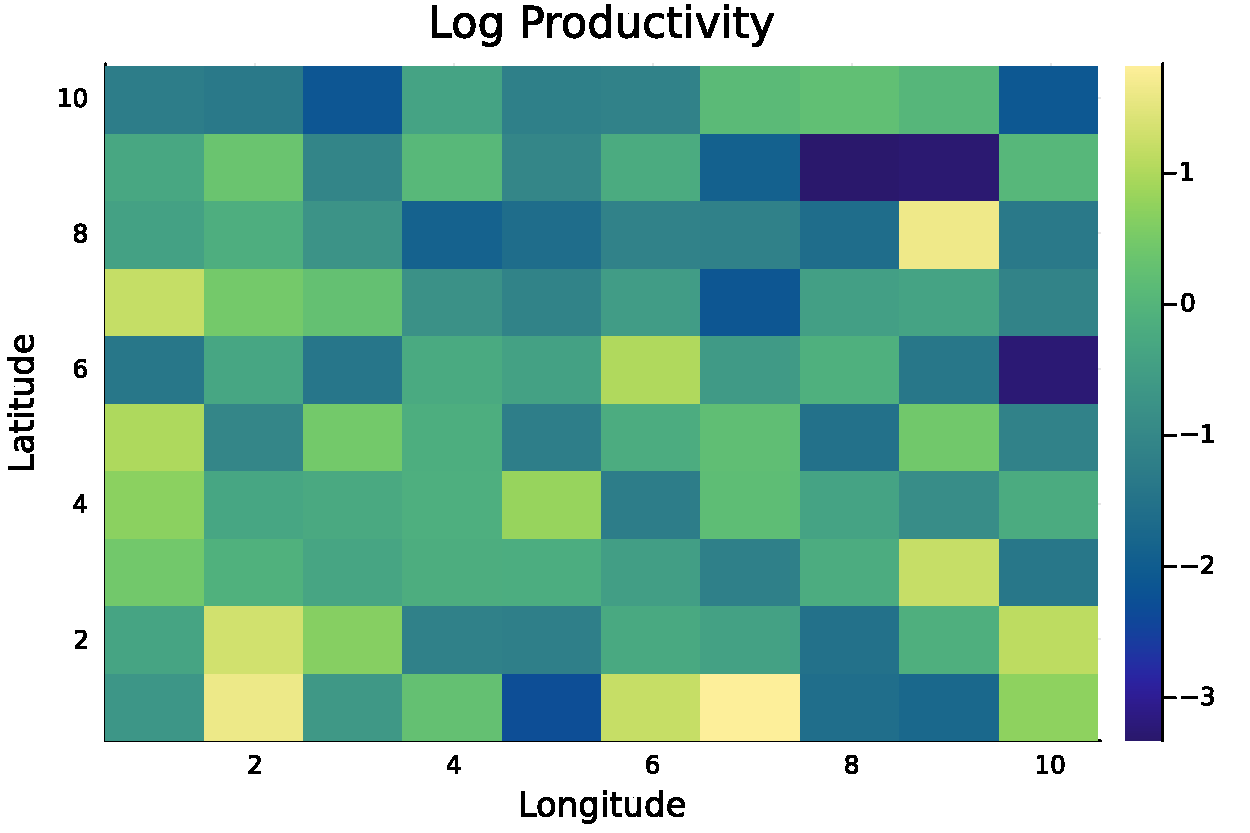
\includegraphics[scale=0.5]{../graph/H_cnty_initial_prod.pdf}
\end{figure}
\item same quality-adjusted land area
\item share of land in residential consumption expenditure $(1 - \alpha ) = 25\%$
\item elasticity of substitution: $\sigma = 5$
\item trade costs are a constant elasticity function of effective distance: $d_{ni} = dist^{\phi}_{ni}$ with $\phi = 0.375$
\item two forms of economic frictions to trade between locations
\begin{enumerate}
\item proportional internal tax on trade with other locations of $100 \%$ ($\tau^{in} = 2$)
\item proportional external tax on trade between the two countries of $100 \%$ ($\tau^{out} = 2$)
\end{enumerate}
\end{itemize}

\subsection*{Initial Equilibrium with both taxes}
Stylized facts from initial equilbirum Figure \ref{initial_equi}:
\begin{itemize}
\item areas of high productivity have large population concentrations, high wages, high land prices
\item log of the price index is a smooth surface with the gradient governed by trade costs
\item prices are lower in areas that produce a large variety of goods, for example, at the two large cities close to the border
\item largest agglomerations in this economy are most clearly appreciated in this panel
\item border effect created by the tariff between the two countries
\end{itemize}

\begin{figure}[H]
\centering
\caption{Initial Equilibrium}
\label{initial_equi}
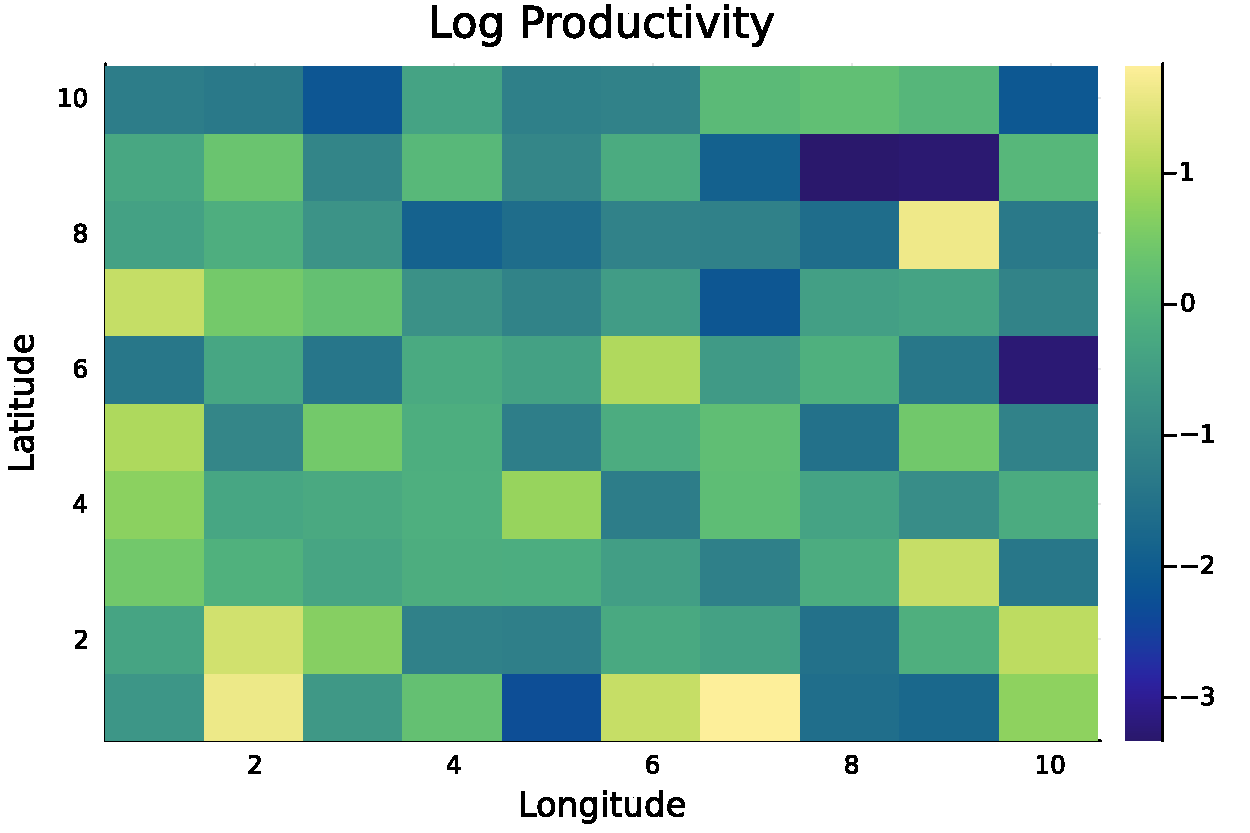
\includegraphics[scale=0.5]{../graph/H_cnty_initial_prod.pdf}
\end{figure}

\subsection*{Counterfactual 1: External Liberalization}
Figure \ref{counter_1} shows the log relative changes ($\hat{x} = x^{'}/x$) in population (log $\hat{L}$), wages (log $\hat{w}$), land prices (log $\hat{r}$), and price indices (log $\hat{P}$) due to removal of the proportional tax on trade between the two countries:
\begin{itemize}
\item as trade costs between the two countries fall, economic activity reallocates toward the border between them
\item areas that benefit the most are the ones close to but on the opposite side of the border from the large cities
\item these locations can now trade more cheaply with the large market in those cities and thus experience the largest increases in population, wages, and land rents and the largest reductions in the price index
\item in contrast, the largest agglomerations lose relative to these up and coming locations
\end{itemize}


\begin{figure}[H]
\caption{External Liberalization: relative changes with respect to the initial equilibrium}
\centering
\label{counter_1}
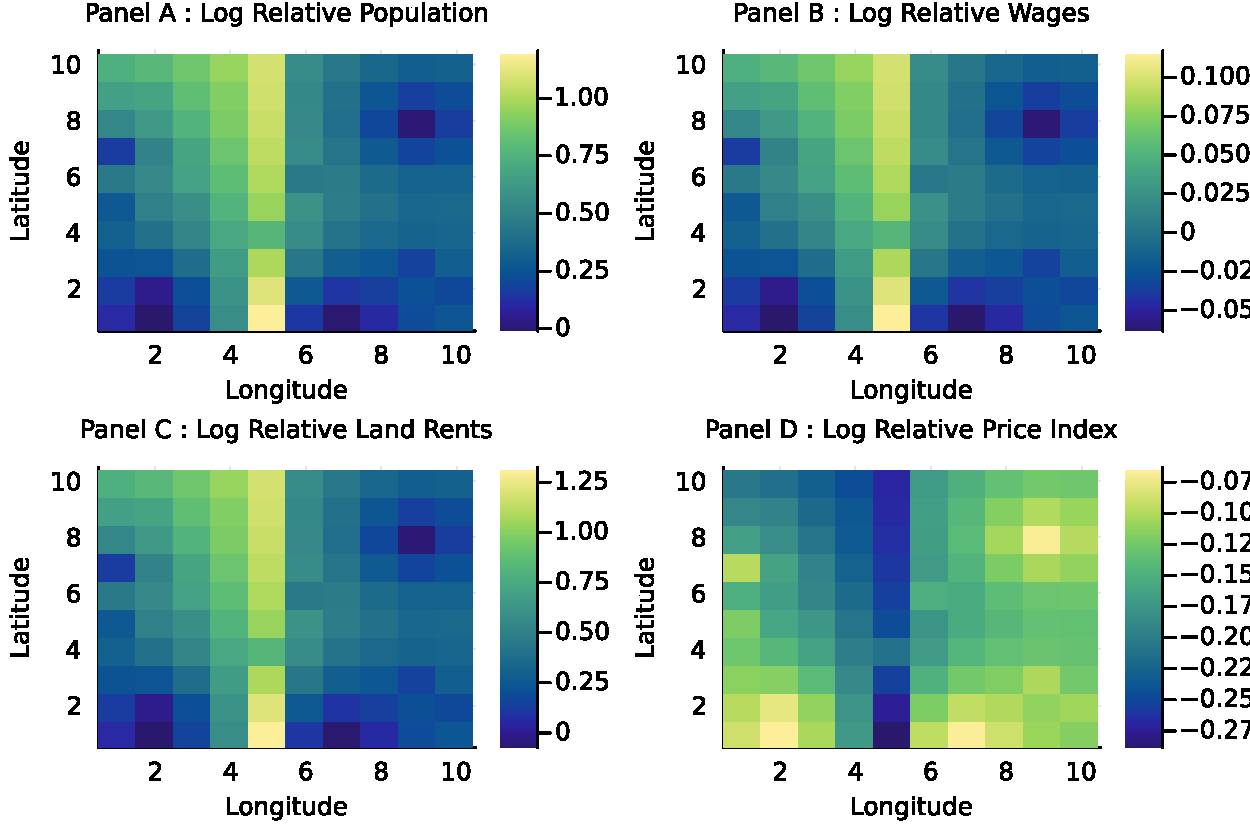
\includegraphics[scale=0.8]{../graph/H_cnty_c.pdf}
\end{figure}

\subsection*{Counterfactual 2: Internal Liberalization}
Figure \ref{counter_2} shows the relative changes with respect to the initial equilibrium ($\hat{x} = x^{'}/x$) due to the removal of all internal trade costs (but leave international trade costs as in the initial equilibrium)
\begin{itemize}
\item implications of an internal reduction in trade costs are clearly quite different than the ones from an external trade cost reduction
\item  main effect of the internal liberalization is to reduce the size of the two large cities in favor of rural areas, thereby making economic activity more dispersed
\item as trade costs decline, the home market effect reducing local price indexes in large cities weakens, so that prices fall everywhere but less so in areas with larger populations
\item wages and land rents also fall in large agglomerations, whereas they increase in all other regions
\end{itemize}

\begin{figure}[H]
\caption{Internal Liberalization: relative changes with respect to the initial equilibrium}
\centering
\label{counter_2}
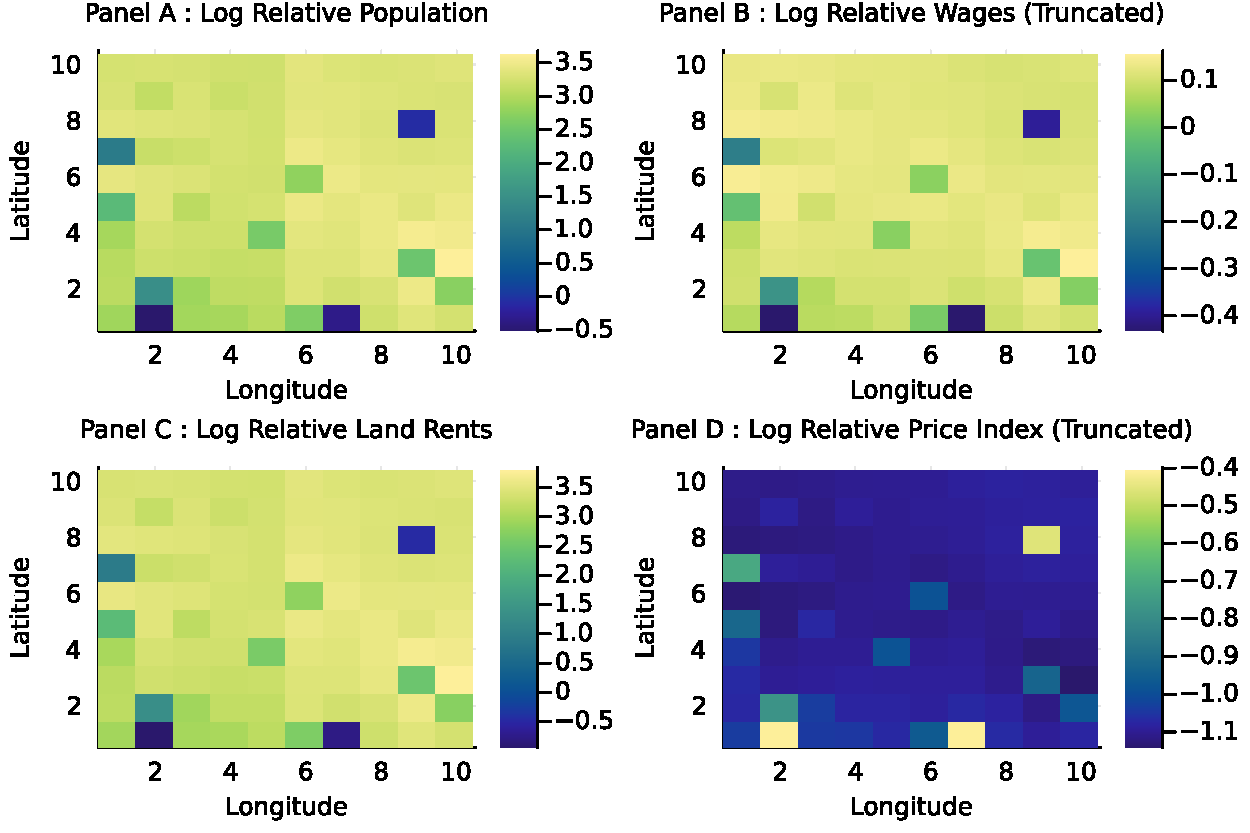
\includegraphics[scale=0.8]{../graph/H_cnty_cc.pdf}
\end{figure}

\subsection*{Welfare Effects of Trade Liberalizations}
Table \ref{welfare} reports the resulting impact (in percentage) of trade liberalization policies on the common level of welfare across locations within each country:
\begin{itemize}
\item internal trade liberalization raises welfare in West and East much higher than external trade liberalization does
\item  trade is much larger between regions than between countries, highlighting the greater importance of internal trade frictions relative to external trade frictions
\end{itemize}

\begin{table}[H]
\centering
\caption{Counterfactuals Welfare gains}
\label{welfare}
\begin{tabular}{lcl}
\toprule 
\multicolumn{3}{c}{Welfare Gains in pct} \\
Trade Liberalization & West & East \\
\midrule 
External & 0.19 & 0.24 \\
\midrule 
Internal & 5.9 & 10.78 \\
\bottomrule 
\end{tabular}

\end{table}

\end{document}